% Created 2016-10-02 Sun 11:19
\documentclass[11pt]{article}
\usepackage[utf8]{inputenc}
\usepackage[T1]{fontenc}
\usepackage{fixltx2e}
\usepackage{graphicx}
\usepackage{longtable}
\usepackage{float}
\usepackage{wrapfig}
\usepackage{soul}
\usepackage{textcomp}
\usepackage{marvosym}
\usepackage{wasysym}
\usepackage{latexsym}
\usepackage{amssymb}
\usepackage{hyperref}
\tolerance=1000
\providecommand{\alert}[1]{\textbf{#1}}

\title{fast-rcnn}
\author{shhs}
\date{\today}
\hypersetup{
  pdfkeywords={},
  pdfsubject={},
  pdfcreator={Emacs Org-mode version 7.9.3f}}

\begin{document}

\maketitle

\setcounter{tocdepth}{3}
\tableofcontents
\vspace*{1cm}

\section{Fast R-CNN --Ross Girshick}
\label{sec-1}


Paper: \href{http://arxiv.org/abs/1504.08083}{Fast R-CNN}
Code: \href{https://github.com/rbgirshick/fast-rcnn}{Fast R-CNN's code}
\subsection{Fast R-CNN architecture and training}
\label{sec-1-1}


   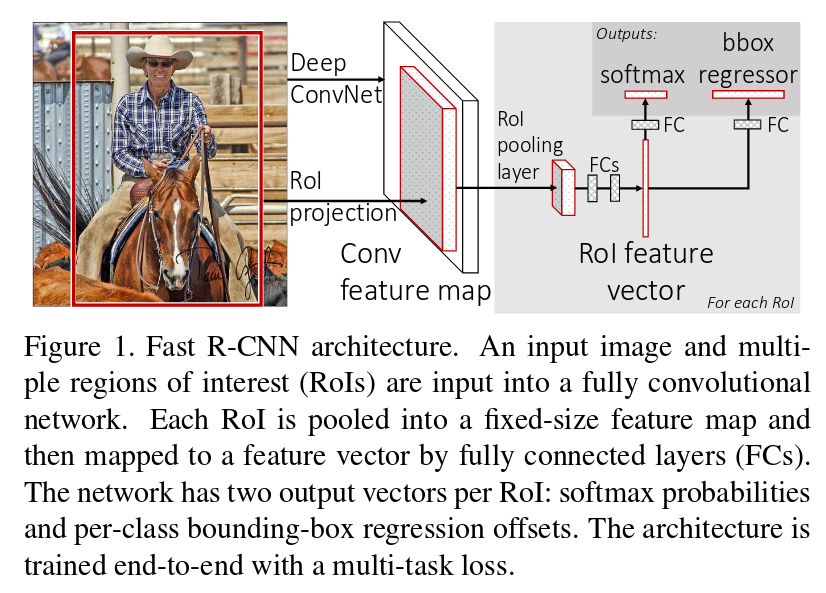
\includegraphics[width=.9\linewidth]{./pic_fast_rcnn/1.png}
\begin{itemize}
\item inputs: \textbf{an entire image}, \textbf{a set of object proposals}
\item several convolutional and max pooling layers -> produce a conv feature map
\item for each object proposal: a RoI(region of interest) pooling layer extracts a 
     fixed-length feature vector from the feature map
\item each feature vector is fed into a sequence of fully connected(fc) layers 
     that finally branch into two sibling(兄弟,姐妹,同属) output layers:
     \textbf{one} that produces softmax probability estimates over K object classes
     plus a catch-all ``background'' class and \textbf{another layer} that outputs 
     four real-valued numbers for each of the K object classes.
\item $\Box$ ? 2. \emph{Each set of 4 values encodes refined bounding-box positions for one of            the K classes.}
\end{itemize}
\subsubsection{The RoI pooling layer}
\label{sec-1-1-1}

\begin{itemize}
\item The RoI pooling layer uses max pooling to convert the features inside any valid
\end{itemize}
    region of interest into a small feature map with a fixed spatial extent of HxW,
    wherer H and W are layer hyper-parameters that are independent of any particular RoI.

\begin{itemize}
\item RoI: (r,c,h,w) specifies its top-left corner(r,c) and its height and width(h,w).
\item RoI max pooling layer divides the hxw RoI window into an HxW grid of sub-windows of
      approximate size h/H x w/W and then max-pooling the values in each sub-window into 
      the corresponding output grid cell.
\end{itemize}
\subsubsection{Initializing from pre-trained networks}
\label{sec-1-1-2}


\begin{itemize}
\item When a pre-trained network initializes a Fast R-CNN network, it undergoes three
      transformations:
\begin{enumerate}
\item The last max pooling layer is replaced by a RoI pooling layer that is configured
         by setting H and W to be compatible with the net's first fully connected layer
         (e.g., H = W = 7 for VGG16).
\item The network's last fully connected layer and softmax are replaced with the two 
         sibling layers described earlier: a fully connected layer and softmax over K + 1
         categories, category-specific bounding-box regressors.
\item The network is modified to take two data inputs: a list of images and a list of
         RoIs in those images.
\end{enumerate}
\end{itemize}
\subsubsection{Fine-tuning for detection}
\label{sec-1-1-3}


\begin{itemize}
\item In Fast R-CNN training, stochastic gradient descent(SGD) mini-batches are sampled 
      hierarchically.
\begin{enumerate}
\item First sampling N images
\item Second sampling R/N RoIs from each image.
\end{enumerate}
\item RoIs from the same image share computation and memory in the forward and backward
      passes.
\item One concern over this strategy is it may cause slow training convergence because
      RoIs from the same image are correlated. This concern does not appear to be a 
      practical issue and we achieve good results with N = 2 and R = 128 using fewer
      SGD iterations than R-CNN.
\end{itemize}
\begin{itemize}

\item Multi-task loss\\
\label{sec-1-1-3-1}%
\begin{itemize}
\item A Fast R-CNN network has two sibling output layers.
\begin{enumerate}
\item The first outputs a discrete probability distribution(per RoI), 
          $p = (p_0, ..., p_K)$, over K + 1 categories.(a softmax over the K + 1 outputs of a
          fully connected layer.
\item The second sibling layer outputs bounding-box regression offsets, 
          $t^k = (t_x^k, t_y^k, t_w^k, t_h^k)$, for each of the K object classes, indexed by k.
\item $\Box$ We use the parameterization for $t^k$ given in \footnote{R. Girshick, J. Donahue, T. Darrell, and J. Malik.  
  Rich feature hierarchies for accurate object detection and semantic segmentation. In CVPR, 2014.
 }, in which t$^k$ specifies a
          scale-invariant translation and log-space height/width shift relative to an object 
          proposal.
\end{enumerate}
\item \textbf{Each trainging RoI} is labeled with a ground-truth class u and a ground-truth bounding-box
       regression target v. We use a multi-task loss L on each labeled RoI to jointly train for
       classification and bounding-box regression:
       \begin{equation}
         L(p, u, t^u, v) = L_{cls}(p, u) + \lambda[u\ge1]L_{loc}(t^u, v)         
       \end{equation}
       in which $L_{cls}(p, u)  = -logp_u$ is log loss for true class u.
\item The second task loss , $L_loc$, is defined over a tuple of true bounding-box regression 
       targets for class u. The Iverson bracket indicator function $[u\ge1]$ evaluates to 1 when 
       $u>1$ and 0 otherwise.For background RoIs there is no notion of a ground-truth bounding box
       and hence $L_{loc}$ is ignored. For bounding-box regression, we use the loss
       \begin{equation}
         L_{loc}(t^u, v) = \sum_{i\in{x, y, w, h}} smooth_{L_1}(t_i^u - v_i)         
       \end{equation}
       in which 
       \begin{equation}
         smooth_{L_1}(x) = 
       \begin{cases}
       {0.5x^2} &\mbox{if |x| < 1}\\
       {|x| - 0.5} &\mbox{otherwise}
       \end{cases}
       \end{equation}
       is a robust $L_1$ loss that is less sensitive to outliers than the $L_2$ loss used in 
       R-CNN and SPPnet.
\begin{itemize}
\item When the regression targets are unbounded, training with $L_2$ loss can require careful
         tuning of learning rates in order to prevent exploding gradients. Eq.3 eliminates this
         sensitivity.
\end{itemize}
\item We normalize the ground-truth regression targets $v_i$ to have zero mean and unit variance.
       All experiments use $\lambda = 1$.
\item \footnote{D. Erhan, C. Szegedy, A. Toshev, and D. Anguelov. 
Scalable object detection using deep neural networks. In CVPR, 2014.
 } uses a related loss to train a class agnostic object proposal network. \footnotemark[2] advocates
       for a two-network system that separates localization and classification.
\item OverFeat\footnote{P. Sermanet,  D. Eigen,  X. Zhang,  M. Mathieu,  R. Fergus,and Y. LeCun.  
OverFeat: Integrated Recognition, Localization and Detection using Convolutional Networks.  
In ICLR,2014.
 }, R-CNN\footnotemark[1], and SPPnet\footnote{K. He, X. Zhang, S. Ren, and J. Sun. 
Spatial pyramid pooling in  deep  convolutional  networks  for  visual  recognition.   
In ECCV, 2014.
 } alse train classifiers and bounding-box 
       localizers, however these methods use stage-wise training, which we show is suboptimal
       for Fast R-CNN.
\end{itemize}


\item Mini-batch sampling\\
\label{sec-1-1-3-2}%
\begin{enumerate}
\item During fine-tuning, each SGD mini-batch is constructed from N = 2 images, chosen uniformly
        at random. We use mini-batches of size R = 128, sampling 64 RoIs from each images.
\item As in \footnotemark[1], we take 25\% of the RoIs from object proposals that have intersection over
        union(IoU) overlap with a ground-truth bounding box of at least 0.5. These RoIs comprise
        the examples labeled with a foreground object class, i.e. $u \ge 1$.
\item The remaining RoIs are sampled from object proposals that have a maximum IoU with ground truth
        in the interval [0.1, 0.5), following \footnotemark[4].
\begin{enumerate}
\item These are the background examples and are labeled with u = 0.
\item The lower threshold of 0.1 appears to act as a heuristic for hard example mining \footnote{P.  Felzenszwalb,  R.  Girshick,  D.  McAllester,  and  D.  Ramanan.   
Object detection with discriminatively trained part based models.
TPAMI, 2010.
 }.
\end{enumerate}
\item During traing, images are horizontally flipped with probability 0.5. No other data 
        augmentation is used.
\end{enumerate}


\item Back-propagation through RoI pooling layers\\
\label{sec-1-1-3-3}%
\begin{enumerate}
\item The RoI pooling layer's backwards function computes partial derivative of the loss
        function with respect to each input variable $x_i$ by following the argmax switches:
        \begin{equation}
          \frac{\partial{L}}{\partial{x_i}} = \sum_r\sum_j[i = i*(r,j)]\frac{\partial{L}}{\partial{y_{rj}}}
        \end{equation}
\begin{itemize}
\item where $x_i\in{R}$ be the i-th activation input into the RoI pooling layer and
\end{itemize}
$y_{rj}$ be the layer's j-th output from the r-th RoI.
\begin{itemize}
\item The RoI pooling layer computes $y_{rj}=x_{i*(r,j)}$, in which $i*(r,j)=argmax_{i^{'}\in{R(r,j)}}x_{i^{'}}$.
\end{itemize}
$R(r,j)$ is the index set of inputs in the sub-window over which the output unit $y_{rj}$ 
        max pools.
\end{enumerate}


\item SGD hyper-parameters\\
\label{sec-1-1-3-4}%
\begin{itemize}
\item The fully connected layers used for softmax classification and bounding-box regression
       are initialized from $N(0,0.01^2)$ and $N(0,0.001^2)$. Biases are initialized to 0.
\item All layers use a pre-layer learning rate of 1 for weights and 2 for biases and a global
       learning rate of 0.001.
\item When training on VOC07 or VOC12 trainval we run SGD for 30k mini-batch iterations, and
       then lower the learning rate to 0.0001 and train for another 10k iterations.
\item Momentum : 0.9 , Parameter decay : 0.0005(on weights and biases)
\end{itemize}

       


\end{itemize} % ends low level
\subsubsection{Scale invariance}
\label{sec-1-1-4}


\begin{enumerate}
\item We explore two ways of achieving scale invariant object detection:
\begin{enumerate}
\item via ``brute force''
\item by using image pyramids
\end{enumerate}
\item These strategies follow the two approaches in \footnotemark[4].
\item Brute-force approach
\begin{itemize}
\item Each image is processed at a pre-defined pixel size during both training and testing.
\item The network must directly learn scale-invariant object detection from the training data.
\end{itemize}
\item Multi-scale approach
\begin{itemize}
\item Provides approximate scale-invariance to the network through an image pyramid.
\item At test-time, the image pyramid is used to approximately scale-normalize each object 
         proposal.
\item During multi-scale training, we randomly sample a pyramid scale each time an image is
         sampled, following \footnotemark[4], as a form of data augmentation.
\end{itemize}
\item We experiment with multi-scale training for smaller networks only, due to GPU memory limits.
\end{enumerate}


          

\end{document}
